\chapter{Átomos y moléculas}\label{ch:g7:atoms-and-molecules}

Toma una gota de agua y córtala en dos. Cada mitad sigue siendo agua.
Corta otra vez una mitad en dos, y otra vez, y otra. ¿Podrías seguir
así para siempre, o llegarías a un trozo tan pequeño que al cortarlo una
vez más obtendrías algo que ya no es agua? Hacia el año 400~a.~C., el
pensador griego Demócrito adivinó la respuesta: la materia está hecha de
piezas diminutas que no se pueden cortar, a las que llamó
\emph{\omterm{def:g7:atoms-and-molecules:atom}{átomos}}, de la palabra griega que significa ``indivisible''. Hicieron
falta más de dos mil años, y el trabajo de los químicos del siglo XIX,
para convertir esa intuición en ciencia. Este capítulo describe esas
piezas, los \omterm{def:g7:atoms-and-molecules:atom}{átomos}, y cómo se agrupan en \omterm{def:g7:atoms-and-molecules:molecule}{moléculas}.

\begin{recall}
Una \omterm{def:g6:pure-substances-and-mixtures:pure-substance}{sustancia pura}, como el agua o el oxígeno, está formada por una
sola \omterm{def:g6:pure-substances-and-mixtures:species}{especie química}; una \omterm{def:g6:pure-substances-and-mixtures:mixture}{mezcla}, como el \omterm{def:g4:air-a-mixture-of-gases:air}{aire}, contiene varias
(\cref{ch:g6:pure-substances-and-mixtures}). El \omterm{def:g4:air-a-mixture-of-gases:air}{aire} tiene unas cuatro
quintas partes de nitrógeno y una quinta parte de oxígeno (\cref{ch:g4:air-a-mixture-of-gases}).
\end{recall}

\section{Los átomos}

\begin{definition}[Átomo]\label{def:g7:atoms-and-molecules:atom}
Toda la materia está construida con partículas extremadamente pequeñas
llamadas
\emph{átomos}\index{atomo@átomo}. En la naturaleza solo hay un centenar de
clases distintas de átomos, y toda sustancia (el agua, el \omterm{def:g4:air-a-mixture-of-gases:air}{aire}, el
hierro, el azúcar, nuestro propio cuerpo) está hecha de átomos de unas
pocas de esas clases.
\end{definition}

\begin{proposition}[Los átomos son diminutos]\label{prop:g7:atoms-and-molecules:tiny}
% ledger: const:a0, earth:diameter (8 cm apple: 12756 km / 8 cm = 1.6 x 10^8;
% 0.1-0.15 nm x 1.6 x 10^8 = 1.7-2.4 cm, a small cherry)
El \omterm{def:g7:atoms-and-molecules:atom}{átomo} más pequeño, el \omterm{def:g7:atoms-and-molecules:atom}{átomo} de hidrógeno, mide alrededor de una
diezmillonésima de milímetro de diámetro; los demás son, como mucho,
unas pocas veces más grandes. Diez millones de \omterm{def:g7:atoms-and-molecules:atom}{átomos} de hidrógeno en
fila formarían una línea de un milímetro. Para imaginarlo: si una
manzana se agrandara hasta el tamaño de la Tierra, cada uno de sus
\omterm{def:g7:atoms-and-molecules:atom}{átomos} tendría más o menos el tamaño de una cereza pequeña.
\end{proposition}

\begin{remark}[Vistos sin ser vistos]\label{rem:g7:atoms-and-molecules:seen}
Ningún microscopio de luz puede mostrar un \omterm{def:g7:atoms-and-molecules:atom}{átomo}: los \omterm{def:g7:atoms-and-molecules:atom}{átomos} son mucho
más pequeños que las ondas de la luz. Desde los años ochenta, unos
microscopios especiales que palpan una superficie con una punta
extremadamente fina han producido imágenes en las que los \omterm{def:g7:atoms-and-molecules:atom}{átomos}
sueltos aparecen como pequeños bultos.
\end{remark}

\begin{definition}[Símbolo de un átomo]\label{def:g7:atoms-and-molecules:symbol}
Cada clase de \omterm{def:g7:atoms-and-molecules:atom}{átomo} tiene un nombre y un \emph{símbolo}\index{simbolo de un atomo@símbolo de un átomo}:
una letra mayúscula, a veces seguida de una letra minúscula. El símbolo
es el mismo en todos los idiomas.
\end{definition}

\begin{center}
\small
\begin{tabular}{llll|llll}
\hline
\omterm{def:g7:atoms-and-molecules:atom}{átomo} & \omterm{def:g7:atoms-and-molecules:symbol}{símbolo} & & color del modelo & \omterm{def:g7:atoms-and-molecules:atom}{átomo} & \omterm{def:g7:atoms-and-molecules:symbol}{símbolo} & & color del modelo \\
\hline
hidrógeno & \ce{H} & \tikz\node[aH]{}; & blanco & sodio & \ce{Na} & \tikz\node[aNa]{}; & morado \\
carbono & \ce{C} & \tikz\node[aC]{}; & negro & azufre & \ce{S} & \tikz\node[aS]{}; & amarillo \\
nitrógeno & \ce{N} & \tikz\node[aN]{}; & azul & cloro & \ce{Cl} & \tikz\node[aCl]{}; & verde \\
oxígeno & \ce{O} & \tikz\node[aO]{}; & rojo & hierro, cobre & \ce{Fe}, \ce{Cu} & & --- \\
\hline
\end{tabular}
\end{center}

\begin{remark}[De dónde vienen los símbolos]\label{rem:g7:atoms-and-molecules:latin}
La mayoría de los \omterm{def:g7:atoms-and-molecules:symbol}{símbolos} son las primeras letras del nombre: \ce{H}
para el hidrógeno, \ce{C} para el carbono, \ce{O} para el oxígeno.
Algunos vienen de un nombre más antiguo, latino: \ce{Na} para el sodio
(\emph{natrium}), \ce{Fe} para el hierro (\emph{ferrum}), \ce{Cu} para
el cobre (\emph{cuprum}). La segunda letra es siempre minúscula: \ce{Co}
es el \omterm{def:g7:atoms-and-molecules:atom}{átomo} de cobalto, mientras que CO, con la O mayúscula, es algo muy
distinto.
\end{remark}

\begin{history}[Los átomos de Dalton, 1808]
En 1808, el químico John Dalton publicó una tabla de los \omterm{def:g7:atoms-and-molecules:atom}{átomos}
conocidos entonces, cada uno dibujado como un pequeño círculo con su
propio signo. Fue el primero en afirmar que todos los \omterm{def:g7:atoms-and-molecules:atom}{átomos} de una
misma clase tienen el mismo peso, y que los químicos podían comparar
esos pesos. Pero también supuso que el agua era un \omterm{def:g7:atoms-and-molecules:atom}{átomo} de hidrógeno
unido a un \omterm{def:g7:atoms-and-molecules:atom}{átomo} de oxígeno; hicieron falta otros cincuenta años para
que los químicos se pusieran de acuerdo en que una \omterm{def:g7:atoms-and-molecules:molecule}{molécula} de agua
contiene \emph{dos} \omterm{def:g7:atoms-and-molecules:atom}{átomos} de hidrógeno.
\end{history}

\begin{omfigure}
\begin{minipage}[b]{0.3\linewidth}\centering
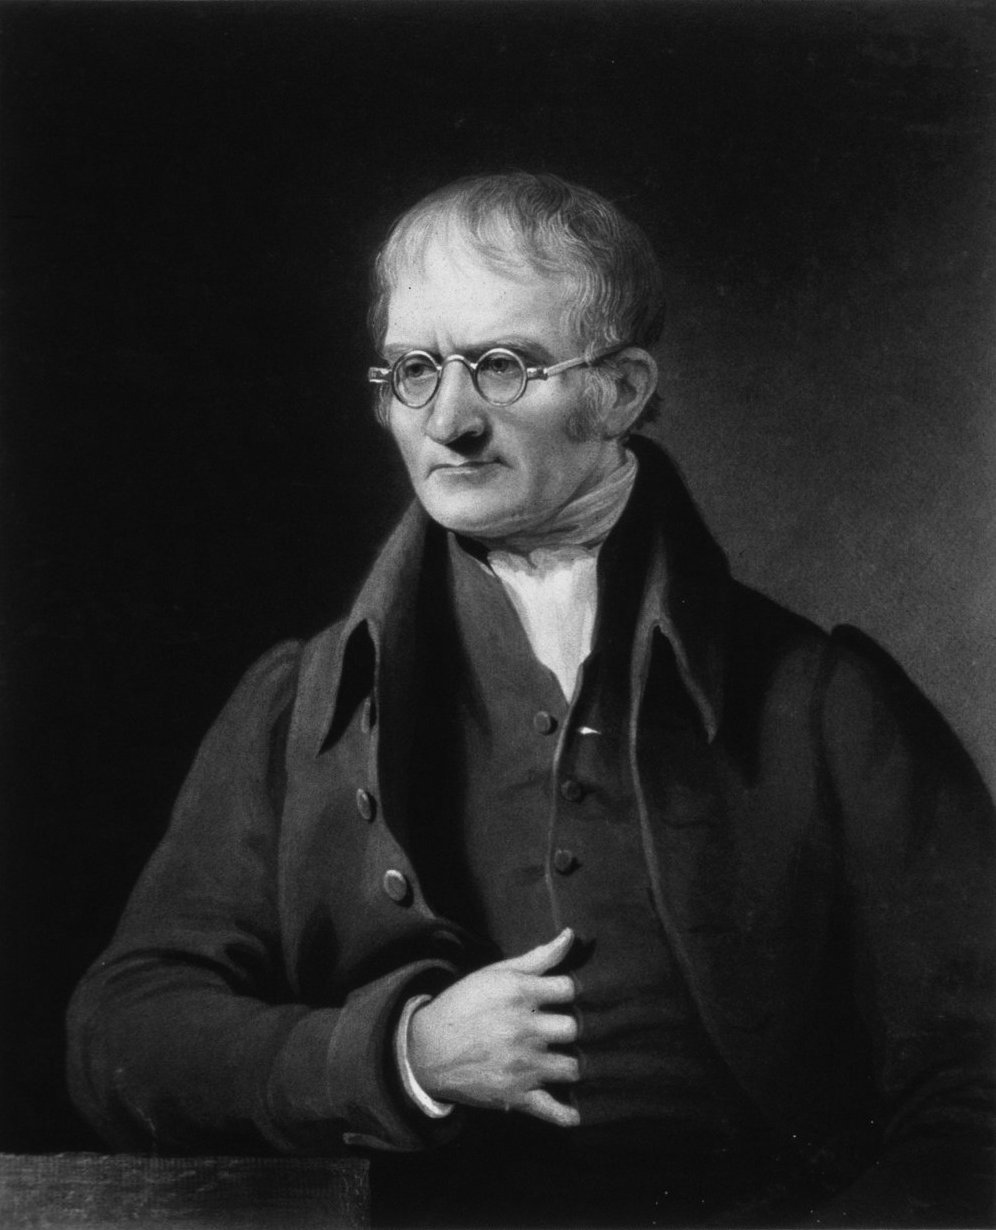
\includegraphics[width=\linewidth]{images/book1/dalton.jpg}

{\small John Dalton (1766--1844).}
\end{minipage}\hfill
\begin{minipage}[b]{0.66\linewidth}\centering
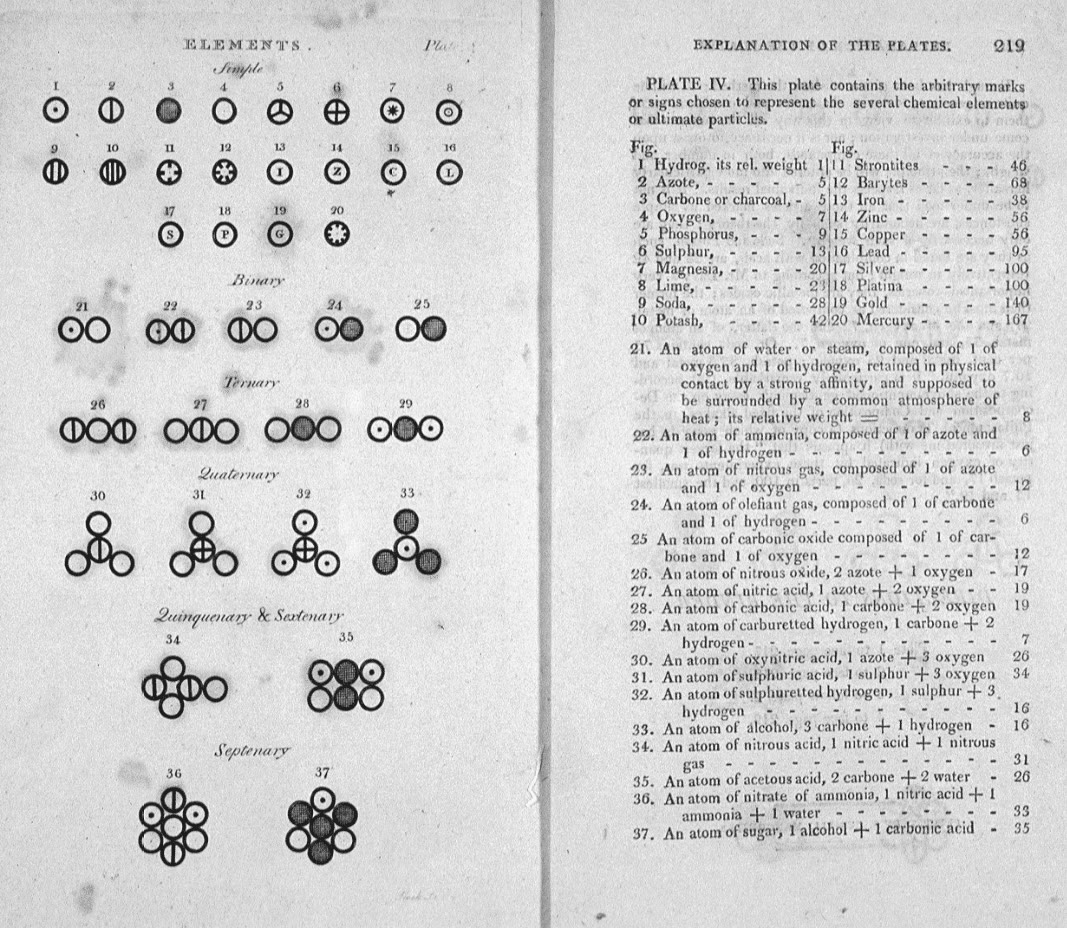
\includegraphics[width=\linewidth]{images/book1/dalton-symbols.jpg}

{\small La tabla de Dalton de 1808: su agua, el signo 21, es un círculo
de hidrógeno junto a uno de oxígeno.}
\end{minipage}
\end{omfigure}

\section{Las moléculas}

\begin{definition}[Molécula]\label{def:g7:atoms-and-molecules:molecule}
Una \emph{molécula}\index{molecula@molécula} es un grupo de \omterm{def:g7:atoms-and-molecules:atom}{átomos} fuertemente
unidos entre sí. Una molécula es el trozo más pequeño de una sustancia
que sigue siendo esa sustancia: una molécula de agua es la cantidad de
agua más pequeña posible.
\end{definition}

\begin{example}[Siete moléculas]\label{ex:g7:atoms-and-molecules:seven}
\begin{itemize}
  \item la \omterm{def:g7:atoms-and-molecules:molecule}{molécula} de \emph{hidrógeno}: dos \omterm{def:g7:atoms-and-molecules:atom}{átomos} de hidrógeno;
  \item la \omterm{def:g7:atoms-and-molecules:molecule}{molécula} de \emph{oxígeno}, que respiramos: dos \omterm{def:g7:atoms-and-molecules:atom}{átomos} de
        oxígeno;
  \item la \omterm{def:g7:atoms-and-molecules:molecule}{molécula} de \emph{nitrógeno}, cuatro quintas partes del \omterm{def:g4:air-a-mixture-of-gases:air}{aire}:
        dos \omterm{def:g7:atoms-and-molecules:atom}{átomos} de nitrógeno;
  \item la \omterm{def:g7:atoms-and-molecules:molecule}{molécula} de \emph{agua}: dos \omterm{def:g7:atoms-and-molecules:atom}{átomos} de hidrógeno y un \omterm{def:g7:atoms-and-molecules:atom}{átomo}
        de oxígeno;
  \item la \omterm{def:g7:atoms-and-molecules:molecule}{molécula} de \emph{dióxido de carbono}, que espiramos: un
        \omterm{def:g7:atoms-and-molecules:atom}{átomo} de carbono y dos \omterm{def:g7:atoms-and-molecules:atom}{átomos} de oxígeno;
  \item la \omterm{def:g7:atoms-and-molecules:molecule}{molécula} de \emph{metano}, la parte principal del gas
        natural que se quema en las cocinas de gas: un \omterm{def:g7:atoms-and-molecules:atom}{átomo} de carbono
        y cuatro \omterm{def:g7:atoms-and-molecules:atom}{átomos} de hidrógeno;
  \item la \omterm{def:g7:atoms-and-molecules:molecule}{molécula} de \emph{óxido de dinitrógeno}, un gas anestésico:
        dos \omterm{def:g7:atoms-and-molecules:atom}{átomos} de nitrógeno y un \omterm{def:g7:atoms-and-molecules:atom}{átomo} de oxígeno.
\end{itemize}
\end{example}

\begin{omfigure}
\begin{tikzpicture}[font=\small]
  % hydrogen
  \begin{scope}[xshift=0cm]
    \node[aH] (a) at (-0.25,0) {}; \node[aH] (b) at (0.25,0) {};
    \begin{scope}[on background layer]\draw[bond] (a.center) -- (b.center);\end{scope}
    \node at (0,-1.05) {hidrógeno};
  \end{scope}
  % oxygen
  \begin{scope}[xshift=2.6cm]
    \node[aO] (a) at (-0.33,0) {}; \node[aO] (b) at (0.33,0) {};
    \begin{scope}[on background layer]
      \draw[bond, line width=1.1pt] ([yshift=1.6pt]a.center) -- ([yshift=1.6pt]b.center);
      \draw[bond, line width=1.1pt] ([yshift=-1.6pt]a.center) -- ([yshift=-1.6pt]b.center);
    \end{scope}
    \node at (0,-1.05) {oxígeno};
  \end{scope}
  % nitrogen
  \begin{scope}[xshift=5.2cm]
    \node[aN] (a) at (-0.33,0) {}; \node[aN] (b) at (0.33,0) {};
    \begin{scope}[on background layer]
      \foreach \d in {-2.4,0,2.4}
        \draw[bond, line width=0.9pt] ([yshift=\d pt]a.center) -- ([yshift=\d pt]b.center);
    \end{scope}
    \node at (0,-1.05) {nitrógeno};
  \end{scope}
  % water
  \begin{scope}[xshift=7.8cm, yshift=0.2cm]
    \node[aO] (o) at (0,0) {};
    \node[aH] (h1) at (-0.62,-0.48) {}; \node[aH] (h2) at (0.62,-0.48) {};
    \begin{scope}[on background layer]
      \draw[bond] (o.center) -- (h1.center); \draw[bond] (o.center) -- (h2.center);
    \end{scope}
    \node at (0,-1.25) {agua};
  \end{scope}
  % carbon dioxide
  \begin{scope}[xshift=0.9cm, yshift=-2.7cm]
    \node[aO] (a) at (-0.85,0) {}; \node[aC] (c) at (0,0) {}; \node[aO] (b) at (0.85,0) {};
    \begin{scope}[on background layer]
      \foreach \d in {-1.6,1.6} {
        \draw[bond, line width=1.1pt] ([yshift=\d pt]a.center) -- ([yshift=\d pt]c.center);
        \draw[bond, line width=1.1pt] ([yshift=\d pt]c.center) -- ([yshift=\d pt]b.center);}
    \end{scope}
    \node at (0,-1.05) {dióxido de carbono};
  \end{scope}
  % methane
  \begin{scope}[xshift=4.4cm, yshift=-2.6cm]
    \node[aC] (c) at (0,0) {};
    \node[aH] (h1) at (0,0.78) {};
    \node[aH] (h2) at (-0.74,-0.3) {};
    \node[aH] (h3) at (0.74,-0.3) {};
    \begin{scope}[on background layer]
      \draw[bond] (c.center) -- (h1.center); \draw[bond] (c.center) -- (h2.center);
      \draw[bond] (c.center) -- (h3.center);
    \end{scope}
    \draw[bond] (c.center) -- (0.22,-0.52);
    \node[aH] at (0.24,-0.58) {};
    \node at (0,-1.15) {metano};
  \end{scope}
  % nitrous oxide
  \begin{scope}[xshift=7.8cm, yshift=-2.7cm]
    \node[aN] (a) at (-0.8,0) {}; \node[aN] (b) at (0,0) {}; \node[aO] (c) at (0.8,0) {};
    \begin{scope}[on background layer]
      \foreach \d in {-1.6,1.6} {
        \draw[bond, line width=1.1pt] ([yshift=\d pt]a.center) -- ([yshift=\d pt]b.center);
        \draw[bond, line width=1.1pt] ([yshift=\d pt]b.center) -- ([yshift=\d pt]c.center);}
    \end{scope}
    \node at (0,-1.05) {óxido de dinitrógeno};
  \end{scope}
\end{tikzpicture}

{\small Modelos de bolas y varillas de las siete \omterm{def:g7:atoms-and-molecules:molecule}{moléculas} del
\cref{ex:g7:atoms-and-molecules:seven}. Cada varilla representa un
enlace entre dos \omterm{def:g7:atoms-and-molecules:atom}{átomos}; por qué algunos \omterm{def:g7:atoms-and-molecules:atom}{átomos} comparten dos o tres
varillas se explica en un capítulo posterior.}
\end{omfigure}

\begin{proposition}[Moléculas de una sustancia pura y de una mezcla]\label{prop:g7:atoms-and-molecules:pure}
En una \omterm{def:g6:pure-substances-and-mixtures:pure-substance}{sustancia pura} formada por \omterm{def:g7:atoms-and-molecules:molecule}{moléculas}, todas las \omterm{def:g7:atoms-and-molecules:molecule}{moléculas} son
idénticas: el agua pura solo contiene \omterm{def:g7:atoms-and-molecules:molecule}{moléculas} de agua. Una \omterm{def:g6:pure-substances-and-mixtures:mixture}{mezcla}
contiene \omterm{def:g7:atoms-and-molecules:molecule}{moléculas} de varias clases: el \omterm{def:g4:air-a-mixture-of-gases:air}{aire} es sobre todo \omterm{def:g7:atoms-and-molecules:molecule}{moléculas} de
nitrógeno y \omterm{def:g7:atoms-and-molecules:molecule}{moléculas} de oxígeno, unas cuatro de nitrógeno por cada una
de oxígeno, con unos pocos \omterm{def:g7:atoms-and-molecules:atom}{átomos} de argón que van sueltos y muy pocas
\omterm{def:g7:atoms-and-molecules:molecule}{moléculas} de dióxido de carbono.
\end{proposition}

\begin{omfigure}
\begin{tikzpicture}[font=\small,
    sN/.style={aN, minimum size=3.0mm}, sO/.style={aO, minimum size=2.9mm},
    sH/.style={aH, minimum size=2.1mm}, sAr/.style={om atom, ball color=cyan!60, minimum size=3.4mm}]
  % air
  \draw[omGlass, line width=0.6pt] (0,0) rectangle (3.4,3.4);
  \foreach \x/\y/\r in {0.5/0.6/20, 1.6/0.4/-30, 2.8/0.7/75, 0.6/1.7/110,
                        2.0/1.5/10, 2.9/2.0/-60, 0.9/2.8/40, 2.1/2.9/-15}
    \node[sN] at ($(\x,\y)+(\r:0.12)$) {} node[sN] at ($(\x,\y)+(\r+180:0.12)$) {};
  \foreach \x/\y/\r in {1.3/1.1/60, 1.6/2.3/-40}
    \node[sO] at ($(\x,\y)+(\r:0.12)$) {} node[sO] at ($(\x,\y)+(\r+180:0.12)$) {};
  \node[sAr] at (2.9,3.0) {};
  \node[anchor=north] at (1.7,-0.1) {\textbf{aire}: una mezcla};
  % water
  \begin{scope}[xshift=5.2cm]
    \draw[omGlass, line width=0.6pt] (0,0) rectangle (3.4,3.4);
    \foreach \x in {0,1,2,3,4} \foreach \y in {0,1,2,3,4} {
      \pgfmathsetmacro{\ang}{mod(73*\x+41*\y,360)}
      \begin{scope}[shift={({0.36+0.67*\x},{0.4+0.66*\y})}, rotate=\ang]
        \node[sH] at (-0.16,-0.12) {}; \node[sH] at (0.16,-0.12) {};
        \node[sO] at (0,0) {};
      \end{scope}}
    \node[anchor=north] at (1.7,-0.1) {\textbf{agua}: una sustancia pura};
  \end{scope}
\end{tikzpicture}

{\small Un zoom enorme. A la izquierda, en el \omterm{def:g4:air-a-mixture-of-gases:air}{aire}, las \omterm{def:g7:atoms-and-molecules:molecule}{moléculas} de
nitrógeno (azules) son muchas más que las de oxígeno (rojas), y un \omterm{def:g7:atoms-and-molecules:atom}{átomo}
de argón (azul claro) viaja solo; las \omterm{def:g7:atoms-and-molecules:molecule}{moléculas} de un gas están muy
separadas. A la derecha, en el agua líquida, las \omterm{def:g7:atoms-and-molecules:molecule}{moléculas} son todas
idénticas y se tocan unas con otras.}
\end{omfigure}

\section{Las fórmulas químicas}

\begin{definition}[Fórmula química]\label{def:g7:atoms-and-molecules:formula}
La \emph{fórmula química}\index{formula quimica@fórmula química} de una \omterm{def:g7:atoms-and-molecules:molecule}{molécula}
enumera los \omterm{def:g7:atoms-and-molecules:symbol}{símbolos} de sus \omterm{def:g7:atoms-and-molecules:atom}{átomos}, cada uno seguido de un número
pequeño escrito por debajo de la línea (el
\emph{subíndice}\index{subindice@subíndice}) que indica cuántos \omterm{def:g7:atoms-and-molecules:atom}{átomos} de esa
clase contiene la \omterm{def:g7:atoms-and-molecules:molecule}{molécula}. El subíndice 1 no se escribe.
\end{definition}

\begin{example}[Las siete fórmulas]\label{ex:g7:atoms-and-molecules:formulas}
Las \omterm{def:g7:atoms-and-molecules:molecule}{moléculas} del \cref{ex:g7:atoms-and-molecules:seven} tienen estas
fórmulas:
\begin{center}
\begin{tabular}{lcl}
\hline
\omterm{def:g7:atoms-and-molecules:molecule}{molécula} & fórmula & \omterm{def:g7:atoms-and-molecules:atom}{átomos} \\
\hline
hidrógeno & \ce{H2} & 2 de hidrógeno \\
oxígeno & \ce{O2} & 2 de oxígeno \\
nitrógeno & \ce{N2} & 2 de nitrógeno \\
agua & \ce{H2O} & 2 de hidrógeno, 1 de oxígeno \\
dióxido de carbono & \ce{CO2} & 1 de carbono, 2 de oxígeno \\
metano & \ce{CH4} & 1 de carbono, 4 de hidrógeno \\
óxido de dinitrógeno & \ce{N2O} & 2 de nitrógeno, 1 de oxígeno \\
\hline
\end{tabular}
\end{center}
\end{example}

\begin{method}[Leer una fórmula]\label{met:g7:atoms-and-molecules:read}
Para leer la fórmula de una \omterm{def:g7:atoms-and-molecules:molecule}{molécula}:
\begin{enumerate}
  \item se divide en \omterm{def:g7:atoms-and-molecules:symbol}{símbolos}: cada uno empieza por una mayúscula;
  \item después de cada \omterm{def:g7:atoms-and-molecules:symbol}{símbolo}, se lee el \omterm{def:g7:atoms-and-molecules:formula}{subíndice} (sin \omterm{def:g7:atoms-and-molecules:formula}{subíndice}
        quiere decir 1);
  \item se suman los \omterm{def:g7:atoms-and-molecules:formula}{subíndices} para obtener el número total de \omterm{def:g7:atoms-and-molecules:atom}{átomos}.
\end{enumerate}
Para \ce{C2H6O} (el etanol, el alcohol de las bebidas): 2 de carbono, 6
de hidrógeno, 1 de oxígeno, 9 \omterm{def:g7:atoms-and-molecules:atom}{átomos} en total.
\end{method}

\begin{remark}[Un número delante]\label{rem:g7:atoms-and-molecules:coefficient}
Un número escrito delante de una fórmula cuenta \omterm{def:g7:atoms-and-molecules:molecule}{moléculas}: \ce{3H2O}
significa tres \omterm{def:g7:atoms-and-molecules:molecule}{moléculas} de agua, que en total contienen 6 \omterm{def:g7:atoms-and-molecules:atom}{átomos} de
hidrógeno y 3 \omterm{def:g7:atoms-and-molecules:atom}{átomos} de oxígeno. No confundas \ce{O2}, una \omterm{def:g7:atoms-and-molecules:molecule}{molécula}
formada por dos \omterm{def:g7:atoms-and-molecules:atom}{átomos} de oxígeno, con \ce{2O}, dos \omterm{def:g7:atoms-and-molecules:atom}{átomos} de oxígeno
que no están unidos.
\end{remark}

\begin{example}[El metano en la cocina]\label{ex:g7:atoms-and-molecules:methane}
El gas natural de una cocina de gas es sobre todo metano, \ce{CH4}. Cada
una de sus \omterm{def:g7:atoms-and-molecules:molecule}{moléculas} es un \omterm{def:g7:atoms-and-molecules:atom}{átomo} de carbono con cuatro \omterm{def:g7:atoms-and-molecules:atom}{átomos} de
hidrógeno a su alrededor. El gas es invisible y no tiene olor: el olor
a ``gas'' es una sustancia que se añade a propósito, para que se note
una fuga.
\end{example}

\begin{omfigure}
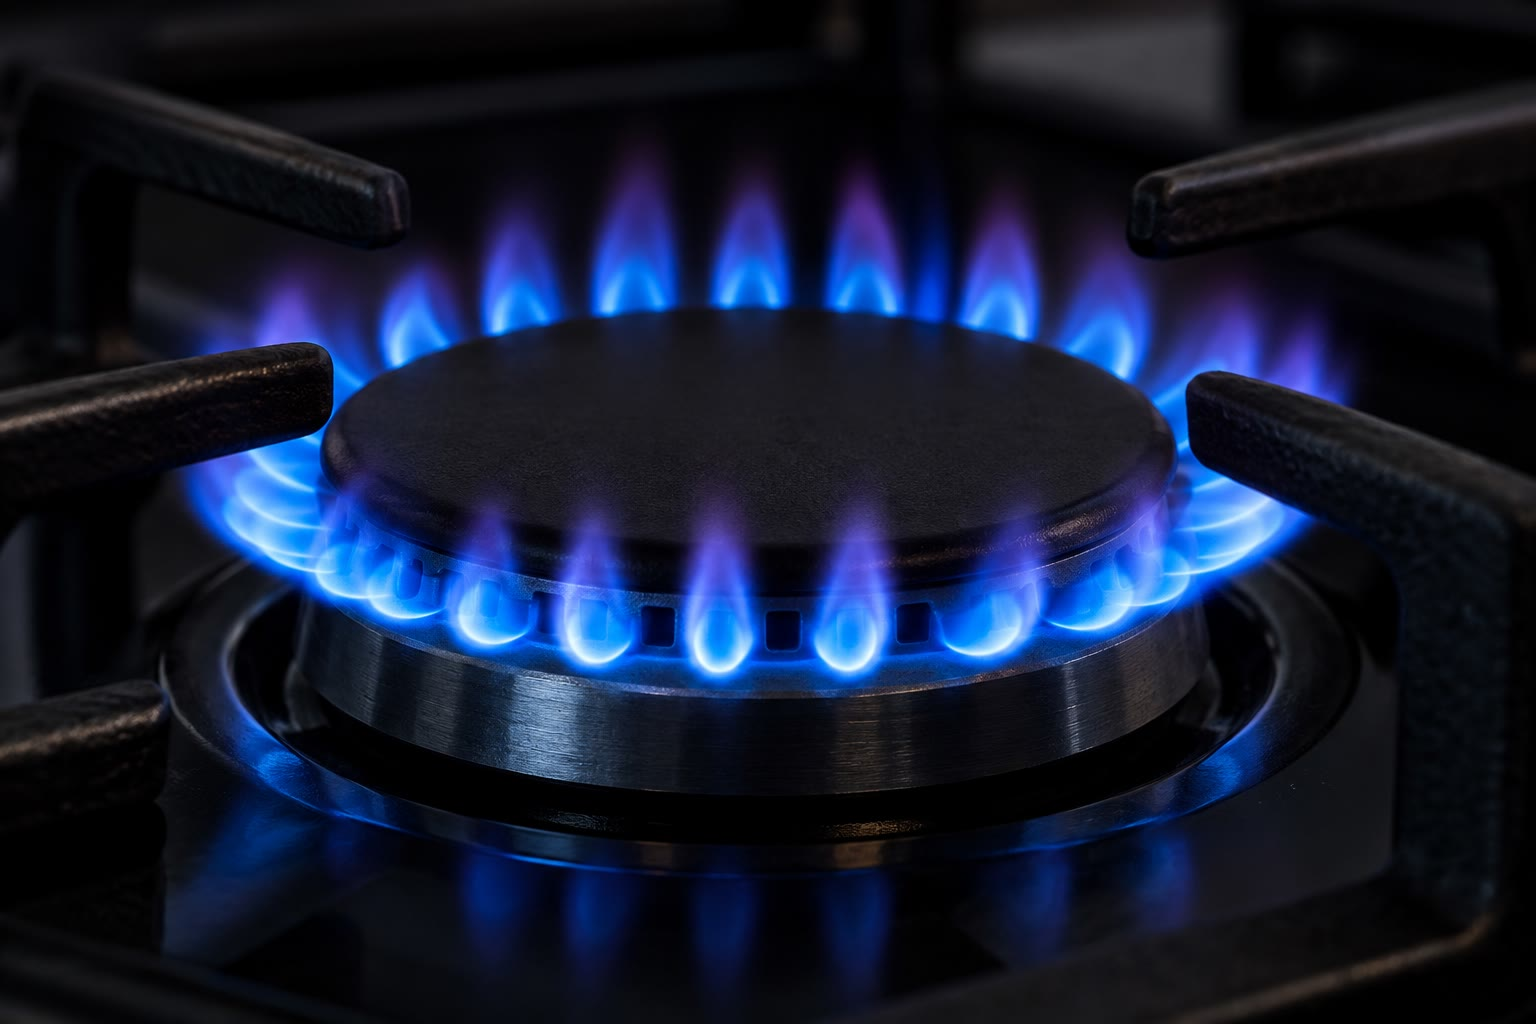
\includegraphics[width=0.5\linewidth]{images/book1/ai/g7-gas-flame.jpg}

{\small La llama azul de una cocina de gas: está \omterm{def:g4:what-a-fire-needs:burning}{ardiendo} el metano del
gas natural.}
\end{omfigure}

\section{Los modelos moleculares}

\begin{remark}[Los modelos y sus colores]\label{rem:g7:atoms-and-molecules:models}
Los químicos construyen \emph{modelos moleculares} con bolas para los
\omterm{def:g7:atoms-and-molecules:atom}{átomos} y varillas para los enlaces entre ellos. Los colores son una
convención que se usa en todo el mundo (carbono negro, hidrógeno blanco,
oxígeno rojo, nitrógeno azul) y no el color real de los \omterm{def:g7:atoms-and-molecules:atom}{átomos}: un \omterm{def:g7:atoms-and-molecules:atom}{átomo}
aislado no tiene ningún color. Un modelo muestra también la forma de una
\omterm{def:g7:atoms-and-molecules:molecule}{molécula}, cosa que una fórmula no hace: la \omterm{def:g7:atoms-and-molecules:molecule}{molécula} de agua es angular,
y la de dióxido de carbono, lineal.
\end{remark}

\begin{omfigure}
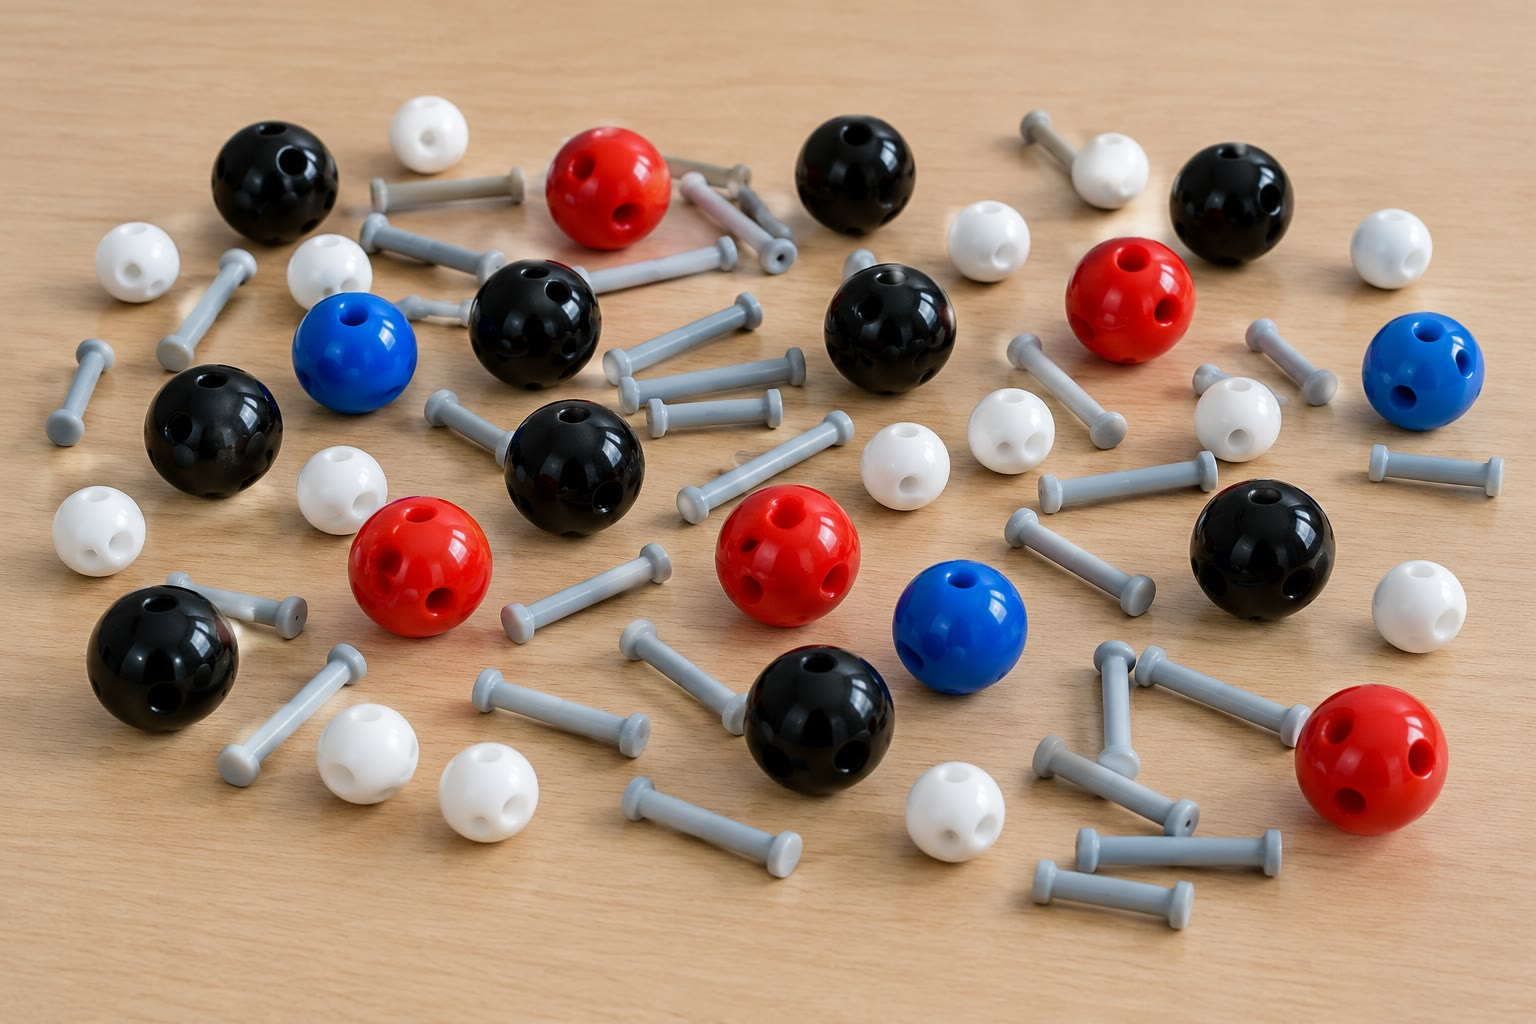
\includegraphics[width=0.5\linewidth]{images/book1/ai/g7-model-kit.jpg}

{\small Un juego de modelos moleculares: bolas para los \omterm{def:g7:atoms-and-molecules:atom}{átomos}, con
agujeros para las varillas que representan los enlaces.}
\end{omfigure}

\begin{method}[De un modelo a una fórmula]\label{met:g7:atoms-and-molecules:model}
Para escribir la fórmula de una \omterm{def:g7:atoms-and-molecules:molecule}{molécula} a partir de su modelo:
\begin{enumerate}
  \item se nombran los \omterm{def:g7:atoms-and-molecules:atom}{átomos} por sus colores;
  \item se cuentan las bolas de cada color;
  \item se escriben los \omterm{def:g7:atoms-and-molecules:symbol}{símbolos} con los recuentos como \omterm{def:g7:atoms-and-molecules:formula}{subíndices}:
        primero el carbono, luego el hidrógeno y después los demás
        \omterm{def:g7:atoms-and-molecules:atom}{átomos} por orden alfabético de sus \omterm{def:g7:atoms-and-molecules:symbol}{símbolos}.
\end{enumerate}
Una bola negra unida a cuatro blancas: un carbono y cuatro hidrógenos,
\ce{CH4}.
\end{method}

\section{Ejercicios}

\begin{exercise}[$\star$]\label{exo:g7:atoms-and-molecules:1}
¿Qué es un \omterm{def:g7:atoms-and-molecules:atom}{átomo}? ¿Qué es una \omterm{def:g7:atoms-and-molecules:molecule}{molécula}?
\end{exercise}

\begin{exercise}[$\star$]\label{exo:g7:atoms-and-molecules:2}
Da los \omterm{def:g7:atoms-and-molecules:symbol}{símbolos} del hidrógeno, el carbono, el nitrógeno, el oxígeno, el
sodio y el hierro.
\end{exercise}

\begin{exercise}[$\star$]\label{exo:g7:atoms-and-molecules:3}
¿Cuántos \omterm{def:g7:atoms-and-molecules:atom}{átomos} de cada clase hay en una \omterm{def:g7:atoms-and-molecules:molecule}{molécula} de dióxido de
carbono, \ce{CO2}? ¿Cuántos \omterm{def:g7:atoms-and-molecules:atom}{átomos} en total?
\end{exercise}

\begin{exercise}[$\star$]\label{exo:g7:atoms-and-molecules:4}
Nombra las \omterm{def:g7:atoms-and-molecules:molecule}{moléculas} \ce{H2O}, \ce{O2}, \ce{CH4} y \ce{N2}.
\end{exercise}

\begin{exercise}[$\star$]\label{exo:g7:atoms-and-molecules:5}
Una \omterm{def:g7:atoms-and-molecules:molecule}{molécula} de dióxido de nitrógeno, un gas pardo que se encuentra en
el \omterm{def:g4:air-a-mixture-of-gases:air}{aire} contaminado, está formada por un \omterm{def:g7:atoms-and-molecules:atom}{átomo} de nitrógeno y dos
\omterm{def:g7:atoms-and-molecules:atom}{átomos} de oxígeno. Escribe su fórmula.
\end{exercise}

\begin{exercise}[$\star\star$]\label{exo:g7:atoms-and-molecules:6}
Explica la diferencia entre \ce{O2} y \ce{2O}, y entre \ce{CO} y
\ce{Co}.
\end{exercise}

\begin{exercise}[$\star\star$]\label{exo:g7:atoms-and-molecules:7}
¿Cuántos \omterm{def:g7:atoms-and-molecules:atom}{átomos} de hidrógeno y cuántos \omterm{def:g7:atoms-and-molecules:atom}{átomos} de oxígeno hay en
\ce{3H2O}? ¿Y en \ce{5O2}?
\end{exercise}

\begin{exercise}[$\star\star$]\label{exo:g7:atoms-and-molecules:8}
Un modelo está formado por una bola negra unida a dos bolas rojas.
Nombra los \omterm{def:g7:atoms-and-molecules:atom}{átomos}, escribe la fórmula y nombra la \omterm{def:g7:atoms-and-molecules:molecule}{molécula}.
\end{exercise}

\begin{exercise}[$\star\star$]\label{exo:g7:atoms-and-molecules:9}
En la tabla de Dalton, el agua está formada por un \omterm{def:g7:atoms-and-molecules:atom}{átomo} de hidrógeno y
un \omterm{def:g7:atoms-and-molecules:atom}{átomo} de oxígeno. Escribe la fórmula que Dalton tenía en mente, y di
cuántos \omterm{def:g7:atoms-and-molecules:atom}{átomos} le faltan a su \omterm{def:g7:atoms-and-molecules:molecule}{molécula} de agua.
\end{exercise}

\begin{exercise}[$\star\star$]\label{exo:g7:atoms-and-molecules:10}
¿Es el agua pura una \omterm{def:g6:pure-substances-and-mixtures:mixture}{mezcla}? ¿Y el \omterm{def:g4:air-a-mixture-of-gases:air}{aire}? Responde describiendo las
\omterm{def:g7:atoms-and-molecules:molecule}{moléculas} que contiene cada uno.
\end{exercise}

\begin{exercise}[$\star\star\star$]\label{exo:g7:atoms-and-molecules:11}
Un \omterm{def:g7:atoms-and-molecules:atom}{átomo} de hidrógeno mide alrededor de una diezmillonésima de milímetro
de diámetro. ¿Cuántos \omterm{def:g7:atoms-and-molecules:atom}{átomos} de hidrógeno, uno al lado del otro,
formarían una línea de \qty{1}{cm}? ¿Y una línea tan larga como un campo
de fútbol, \qty{100}{m}?
\end{exercise}

\begin{exercise}[$\star\star\star$]\label{exo:g7:atoms-and-molecules:12}
La glucosa, el azúcar que alimenta nuestras células, tiene la fórmula
\ce{C6H12O6}. ¿Cuántos \omterm{def:g7:atoms-and-molecules:atom}{átomos} contiene una \omterm{def:g7:atoms-and-molecules:molecule}{molécula} de glucosa? ¿Qué
porcentaje de ellos son \omterm{def:g7:atoms-and-molecules:atom}{átomos} de hidrógeno? ¿Qué porcentaje son \omterm{def:g7:atoms-and-molecules:atom}{átomos}
de carbono?
\end{exercise}

\section{Problema: Los átomos de una respiración}

\begin{problem}[{Problema de fin de semana --- contar los átomos de una
bocanada de aire, antes y después de pasar por nuestros pulmones}]
\label{pb:g7:atoms-and-molecules:1}
% ledger: air:N2, air:O2, air:Ar (78.08 / 20.95 / 0.93 rounded to 78 / 21 / 1),
% breath:O2, breath:CO2, breath:N2 (expired air: 16 / 4 / 78, water vapour removed)
El nitrógeno atraviesa los pulmones sin cambiar, así que sirve de
referencia. En el \omterm{def:g4:air-a-mixture-of-gases:air}{aire} seco, por cada 78 \omterm{def:g7:atoms-and-molecules:molecule}{moléculas} de nitrógeno hay unas
21 \omterm{def:g7:atoms-and-molecules:molecule}{moléculas} de oxígeno y 1 \omterm{def:g7:atoms-and-molecules:atom}{átomo} de argón: 100 partículas (\omterm{def:g7:atoms-and-molecules:molecule}{moléculas} o
\omterm{def:g7:atoms-and-molecules:atom}{átomos} sueltos) en total. En el \omterm{def:g4:air-a-mixture-of-gases:air}{aire} espirado, una vez eliminado su
vapor de agua, las mismas 78 \omterm{def:g7:atoms-and-molecules:molecule}{moléculas} de nitrógeno van acompañadas de
unas 16 \omterm{def:g7:atoms-and-molecules:molecule}{moléculas} de oxígeno, 4 \omterm{def:g7:atoms-and-molecules:molecule}{moléculas} de dióxido de carbono y 1
\omterm{def:g7:atoms-and-molecules:atom}{átomo} de argón.

\medskip
\noindent\textbf{Parte I --- El \omterm{def:g4:air-a-mixture-of-gases:air}{aire} que inspiramos.}
\begin{enumerate}
  \item Escribe las fórmulas de las \omterm{def:g7:atoms-and-molecules:molecule}{moléculas} de nitrógeno, de oxígeno y
        de dióxido de carbono, y da el número de \omterm{def:g7:atoms-and-molecules:atom}{átomos} de cada una.
  \item El argón se cuenta en \omterm{def:g7:atoms-and-molecules:atom}{átomos}, no en \omterm{def:g7:atoms-and-molecules:molecule}{moléculas}. ¿Qué nos dice
        esto sobre el argón?
  \item En estas 100 partículas de \omterm{def:g4:air-a-mixture-of-gases:air}{aire} inspirado, ¿cuántos \omterm{def:g7:atoms-and-molecules:atom}{átomos} de
        nitrógeno hay? ¿Cuántos \omterm{def:g7:atoms-and-molecules:atom}{átomos} de oxígeno?
  \item ¿Cuántos \omterm{def:g7:atoms-and-molecules:atom}{átomos} hay en total en estas 100 partículas?
  \item ¿Qué porcentaje de estos \omterm{def:g7:atoms-and-molecules:atom}{átomos} son \omterm{def:g7:atoms-and-molecules:atom}{átomos} de nitrógeno?
        Redondea al número entero más próximo.
\end{enumerate}

\medskip
\noindent\textbf{Parte II --- El \omterm{def:g4:air-a-mixture-of-gases:air}{aire} que espiramos.}
\begin{enumerate}[resume]
  \item En el \omterm{def:g4:air-a-mixture-of-gases:air}{aire} espirado que acompaña a las mismas 78 \omterm{def:g7:atoms-and-molecules:molecule}{moléculas} de
        nitrógeno, ¿cuántos \omterm{def:g7:atoms-and-molecules:atom}{átomos} de oxígeno hay dentro de \omterm{def:g7:atoms-and-molecules:molecule}{moléculas} de
        oxígeno? ¿Y dentro de \omterm{def:g7:atoms-and-molecules:molecule}{moléculas} de dióxido de carbono? ¿Y en
        total?
  \item Compara con la pregunta 3. ¿Cuántos \omterm{def:g7:atoms-and-molecules:atom}{átomos} de oxígeno faltan?
        ¿En qué \omterm{def:g7:atoms-and-molecules:molecule}{molécula}, fabricada en el cuerpo a partir del hidrógeno
        de los alimentos y eliminada aquí con el vapor de agua, han
        acabado?
  \item ¿Cuántos \omterm{def:g7:atoms-and-molecules:atom}{átomos} de carbono hay en el \omterm{def:g4:air-a-mixture-of-gases:air}{aire} inspirado? ¿Y en el
        \omterm{def:g4:air-a-mixture-of-gases:air}{aire} espirado?
  \item El \omterm{def:g4:air-a-mixture-of-gases:air}{aire} no lleva \omterm{def:g7:atoms-and-molecules:atom}{átomos} de carbono a los pulmones. ¿De dónde
        pueden venir los \omterm{def:g7:atoms-and-molecules:atom}{átomos} de carbono del aliento? (Piensa en lo
        que usa el cuerpo para vivir.)
  \item ¿Cuántas \omterm{def:g7:atoms-and-molecules:molecule}{moléculas} de oxígeno han desaparecido, y cuántas
        \omterm{def:g7:atoms-and-molecules:molecule}{moléculas} de dióxido de carbono han aparecido?
\end{enumerate}

\medskip
\noindent\textbf{Parte III --- El recuento.}
\begin{enumerate}[resume]
  \item Describe el modelo de bolas y varillas de cada una de las cuatro
        clases de partículas del \omterm{def:g4:air-a-mixture-of-gases:air}{aire} espirado, con los colores de las
        bolas (el argón se representa con una sola bola azul claro).
  \item ¿Cuántos \omterm{def:g7:atoms-and-molecules:atom}{átomos} hay en total en el \omterm{def:g4:air-a-mixture-of-gases:air}{aire} espirado seco? ¿Cuántos
        \omterm{def:g7:atoms-and-molecules:atom}{átomos} más que en el \omterm{def:g4:air-a-mixture-of-gases:air}{aire} inspirado? Explica la diferencia con
        los \omterm{def:g7:atoms-and-molecules:atom}{átomos} de carbono ganados y los \omterm{def:g7:atoms-and-molecules:atom}{átomos} de oxígeno que
        faltan.
\end{enumerate}
\end{problem}
